\documentclass[DM,lsstdraft,toc,usenatbib]{lsstdoc}

% Package imports go here
\usepackage{amsmath}	% Advanced maths commands
\usepackage{amssymb}
\usepackage{gensymb}  % degree symbol 
\usepackage{natbib}  % bibliography
\usepackage{cprotect} 
\usepackage{longtable} % for 'longtable' environment
\usepackage{pdflscape} % for 'landscape' environment

% Local commands go here

%% Journal abbreviations
%\bibliographystyle{aasjournal}

\title[Crowded fields ]{LSST  Crowded Fields photometry}

\author{
K.~Suberlak, C.~Slater, \v{Z}.~Ivezi\'c}

\setDocRef{LSST-2017}
\date{\today}
\setDocRevision{TBD}
\setDocStatus{draft}
\setDocAbstract{
A report on the performance of current LSST Stack pipelines in crowded stellar fields. We use the DECAPS data to define the photometry and astrometry quality assurance metrics. 

% 644035
In the top 10\% region, where DECAPS detects 200 000 sources per sq.deg., the mean LSST-DECAPS completeness in 18-20 mag is 80\%, and it drops to 50\% at 21.5 mag. For the same visit, the DECAPS $5\sigma$ limiting depth is 23 mag. 

% 566793 
For a top 2\% region, within the exclusion zone, in which DECAPS detects 500 000 sources per sq.deg., the mean completeness in 18-20 mag of LSST to DECAPS source-by-source is 78\%, and it drops to 50\% at 20.2 mag.  For the same visit, the DECAPS $5\sigma$ limiting depth is 23.2 mag. 


The systematic offset in photometry  (the difference between the median photometric uncertainty and the measure of internal photomtric repeatability) at 21 mag for the density of 200 000 sources per sq.deg.  is 0.06 mag. 

% here we refer to Fig. 22
The LSST photometry is consistent with DECAPS. Above 19th mag, LSST and DECAPS are in systematics-dominated regime, consistent at 0.02 mag level. At fainter magnitudes, the scatter between LSST and DECAPS is less than the photometric uncertainty. 

% here we refer to Fig. 27
The spread of astrometric repeatability  for LSST  epoch-to-epoch is at the level of 10-30 miliarcsec, and is not strongly dependent on stellar crowdedness. 
}

% ### Change history defined here. Will be inserted into
% correct place with \maketitle
% OLDEST FIRST: VERSION, DATE, DESCRIPTION, OWNER NAME
\setDocChangeRecord{%
\addtohist{1}{2018-03-20}{Final draft.}{Krzysztof Suberlak}
}

\begin{document}

% Create the title page
% Table of contents will be added automatically if "toc" class option
% is used.
\maketitle

\section{Introduction}

We report on the performance of the Large Scale Synoptic Telescope (LSST) science pipelines\footnote{\url{https://pipelines.lsst.io}}, also known as 'the LSST stack', in the stellar fields of varying levels of source crowdedness.

The LSST will sample every night on average over 500  regions in the sky , delivering terabytes of raw data in need of processing, including photometric  and astrometric calibration, to deliver a calibrated exposure image, as well as a source catalog, among image products\footnote{\url{http://ls.st/LSE-163}}~\cite{narayan2018}.

The survey sky is composed of regions very diverse in terms of stellar density, or crowdedness. Assuming the single-visit depth of 24.5 mag, the stellar density ranges from high density low-galactic latitude regions that have tens of millions of sources per square degree, to low-density regions towards the Galactic poles with less than thousand sources per square degree. 

Deblending and successful photometry is an inherent part of any astronomical data processing pipeline.  There exists a body of research answering questions that are specific to crowded stellar fields, eg. how many beams do we need per source ~\citep{hogg2001}, or how  the crowded fields photometry can be approached in the era of large telescopes ~\cite{olsen2003}. Other studies involving HyperSuprime CAM pipeline ( developed in parallel with the LSST Stack) recognized that the deeper the survey, the higher the stellar densities encountered, and therefore, the more challenging the process of deblending photometry~\cite{bosch2017}.

In this report we compare the 'out-of-the-box' LSST Stack processing pipeline, to the DECAm [Galactic] Plane Survey (DECAPS) pipeline deveolped by Schlafly et al.~\cite{schlafly2017}. 

To test performance of pipelines at different levels of stellar crowdedness, we choose regions of the sky at various densities based on the Galfast simulation of the night sky (Sec.~\ref{sec:MAF}). 

Given the expected stellar density as a function of position on the sky, we selected DECAPS fields, and processed them with LSST pipelines (Sec.~\ref{sec:DECAPS}). 

We compare the results of the LSST and DECAPS processing of the same visits by cross-matching the catalogs and comparing source counts, photometry (Sec.~\ref{sec:LSST}), and astrometry (Sec.~\ref{sec:astrometry}). We summarize the key results and suggest future work in Sec.~\ref{sec:conclusions}. 



% #############################################################
% ########################## MAF  ############################
% #############################################################

\section{Identifying density regions}
\label{sec:MAF}
To identify regions representing different stellar densities we use the Galfast simulated stellar density map  
prepared as part of Metrics Analysis Framework\footnote{\url{https://www.lsst.org/scientists/simulations/maf}} by P. Yoachim and L. Jones\footnote{\url{sims_maf/python/lsst/sims/maf/maps/createStarDensitymap.py}}.

The  resulting dataset describes the simulated sky, divided into 49152 healpixels. Each healpixel contains 64 magnitude bins between 15 and 28 mag, each bin storing the cumulative count of sources per square degree\footnote{Healpix stands for Hierarchical Equal Area isoLatitude Pixelization\url{http://healpix.sourceforge.net}\citep{gorski2005}}. We select the bin corresponding to the LSST single-visit depth of r=24.5. For each healpixel we find the fraction of pixels that have a higher stellar count (see Fig.~\ref{fig:MAF_densities}).



\begin{figure}
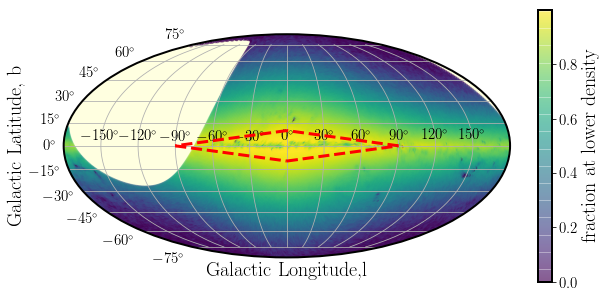
\includegraphics[width=1.0\columnwidth]{figs/MAF_densities.png}
%\vskip -0.15in
\caption{Galfast healpixels plotted in galactic coordinates in Mollweide projection. The brightest regions correspond to highest stellar densities. The missing part at  $\delta>40 \degree$  is not observable from the southern location of Cerro Pach\'on, hence excluded from the simulation. The red dashed lines outline the galactic exclusion zone. }
\label{fig:MAF_densities}
\end{figure} 

Since by definition each healpixel has an equal area, the fraction of pixels  corresponds to the fraction of the sky area. We choose to describe the level of stellar crowdedness by the percentage of the sky that has a higher density. Thus eg.  '5\%' density means that only 1 in 100 pixels has a higher density (see Fig.~\ref{fig:illustrate_density}). Fig.~\ref{fig:mollw_galactic} shows thus defined density brackets in Galactic coordinates.

\begin{figure}
\centering
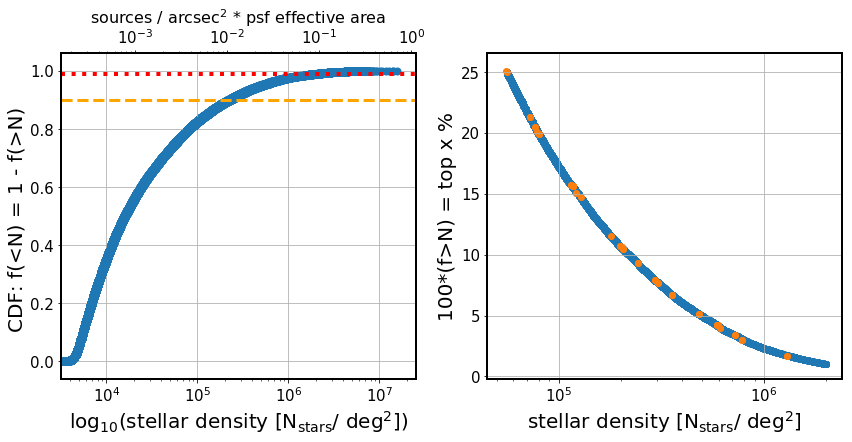
\includegraphics[width=0.95\columnwidth]{figs/MAF_density_definitions.png}
\vskip -0.15in
\caption{Using the Galfast sky simulation to choose DECAPS fields sampling different density regions.  The left panel shows the fraction of the sky at a smaller density  as a function of  the stellar density.  It is equivalent to the cumulative area of the sky up to given density. Given the stellar density per simulated healpixel, we count the number of healpixels at greater density. Normalized to the number of pixels, given their equal area, it corresponds to the fraction of the sky at greater stellar density. Horizontal dashed lines illustrate selecting pixels at top 1\% or 10\% density. The right panel focuses on the top 25\% of density.  It implies that according to the simulation , the density of 200 000 stars per sq.deg. corresponds to 5\% of the sky, and only  1\% of the sky has more than 1 mln stars per sq.deg. The upper axis represents the dimensionless density parameter $N_{beam} = N_{stars}/{arcsec}^{2} * A_{PSF}$, with the PSF effective area $A_{PSF} = 0.64$ \arcsec.}
\label{fig:illustrate_density}
\end{figure} 


\begin{figure}
\centering
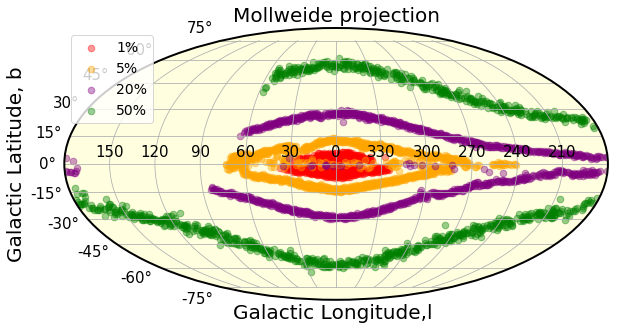
\includegraphics[width=0.9\columnwidth]{figs/03_density_regions_mollw_galactic.png}
\vskip -0.15in
\caption{Regions representative of different simulated stellar densities. The x\%  denotes  x $\pm$ 1\%, eg.  5\% includes regions between 4-6\%. The highest density regions are located close to the galactic bulge, and regions of approximately constant stellar density trace isophotes of the Milky Way. The few 20\% regions close to the galactic equator correspond to high extinction regions that appear to have less counts due to interstellar dust. The galactic exclusion zone in LSST is closely follows the 5\% region outline (see Fig.\ref{fig:MAF_densities}).}
\label{fig:mollw_galactic}
\end{figure} 


% ###############################################################
% ########################## DECAPS  ############################
% ###############################################################

\section{DECam Plane Survey }
\label{sec:DECAPS}
To test the performance of the LSST Stack with real data, we used the Dark Energy Camera (DECam) imaging, taken as part of the  DECam Plane Survey (DECAPS)~\cite{schlafly2017}, at the 4-m Cerro Tololo Inter-American Observatory telescope (CTIO)\footnote{see \url{http://www.ctio.noao.edu/noao/node/1033}}. Each DECAPS image plane is tiled by a mosaic of 62 CCDs, each  2046x4094 px, 0.27 \arcsec/px\footnote{See Fig.4-3 in the NOAO Data Handbook ~\citep{shaw2015}}. The FOV of full mosaic is 2.2\degree  wide -  several times bigger than the full moon - which makes it comparable to the LSST 3.5\degree field of view.  All DECAPS single-epoch images were processed with the DECAPS pipeline, resulting in single-epoch catalogs\footnote{All available via \url{http://decaps.skymaps.info/catalogs.html}}. The details of DECAPS pipeline can be found in Schlafly et al. 2017~\cite{schlafly2017}, but it was specifically designed for crowded field photometry,  performing DAOPhot-like procedure~\cite{stetson1987}, without employing DAOPhot. The algorithm performs repeated source detection, subtraction, and re-detection, which is different from the LSST pipeline. DECAPS pipeline simultaneously solves for the positions and fluxes for all stars for a small fragment of the CCD (see Sec.4 in ~\cite{schlafly2017}).  The headers of all DECAPS catalogs,  assembled into the image database with information about single-visit exposure time, filter,  time of observation, position, were  
used to select fields in  u,g,r  filter, with exposure between 90 and 120 sec (to match the LSST 30 sec single-visit depth in r). Of these, we chose visits representative of given stellar densities based on the Galfast simulation (see Fig.~\ref{fig:decaps_fields}).  Postage stamp miniatures (Fig.~\ref{fig:decaps_illustrate}) show that we indeed sample vastly diffferent densities. Comparing DECAPS to Galfast counts (Fig.~\ref{fig:maf_decaps_counts}) we find that although the simulation may be not more accurate than up to a actor of a few, it is nevertheless useful for defining density regions. 

\begin{figure}

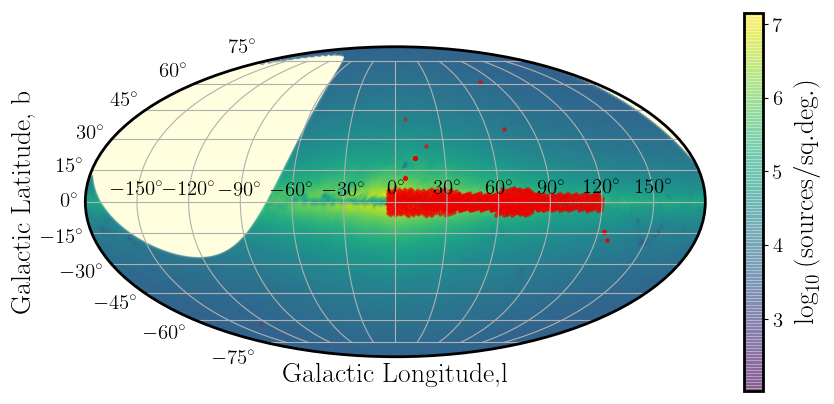
\includegraphics[width=1.0\columnwidth]{figs/MAF_DECAPS.png}
%\vskip -0.15in
\caption{DECAPS fields (red) plotted on top of the Galfast simulated stellar density map (counts up to r<24.5). Cross-matching DECAPS catalog to Galfast simulation we selected visits representative of diverse range of stellar densities.}
\label{fig:decaps_fields}
\end{figure} 


\begin{figure}
\begin{centering}
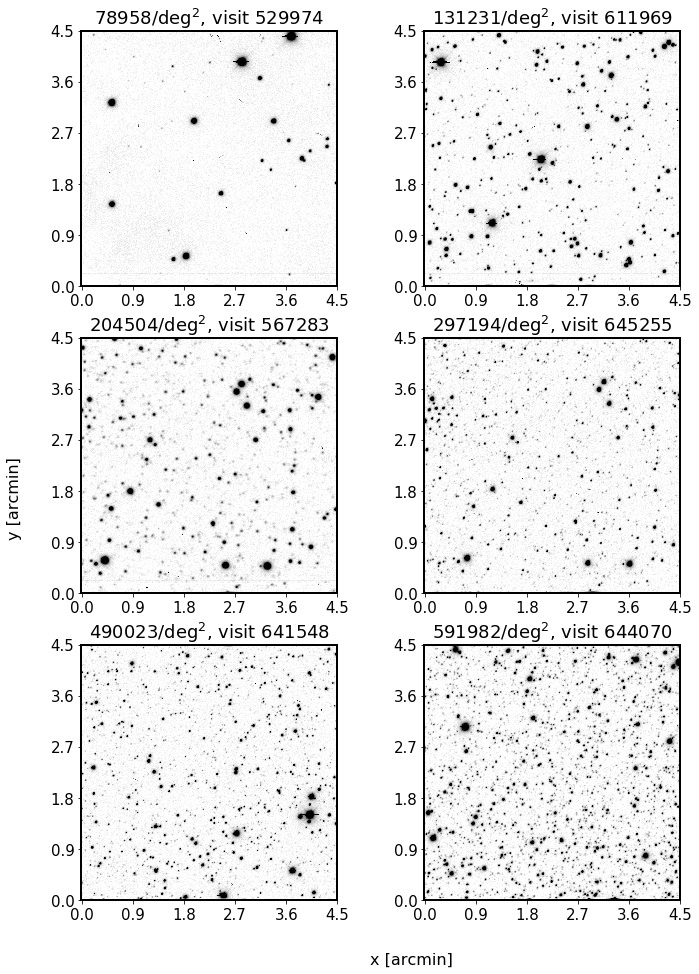
\includegraphics[width=0.85\columnwidth]{figs/Illustrate_densities_DECAPS.png}
\vskip -0.15in
\caption{Illustration of regions of different stellar count in the cleaned DECAPS single-epoch catalogs. As shown on Fig.~\ref{fig:maf_decaps_counts}, the Galfast count does not always correspond 1:1 to the DECAPS stellar count. For this reason we ordered DECAPS fields in terms of DECAPS source count rather than Galfast densities.}
\label{fig:decaps_illustrate}
\end{centering}
\end{figure} 


\begin{figure}
\centering
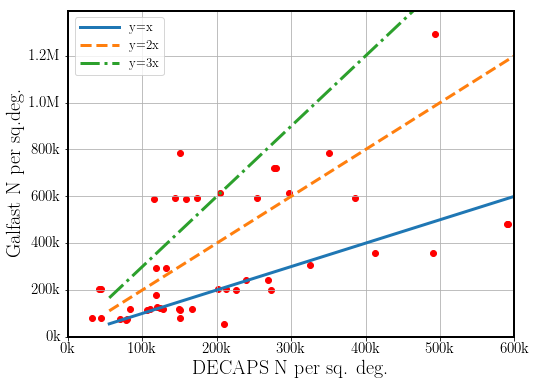
\includegraphics[width=0.75\columnwidth]{figs/MAF_DECAPS_comparison.png}
%\vskip -0.15in
\caption{Comparison of DECAPS counts to Galfast simulated stellar counts.  Overplotted are the line of equivalence y=x, and its multipicities (2x,3x). Part of the reason for discrepancy could be the order-of-magnitude nature of the experiment - Galfast counts here assume the single-visit depth of 24.5 mag in r-band. The DECAPS exposure time ($\approx$100 sec) and filter (g, or r) were chosen to mimic that depth as closely as possible, but the regions targeted include much extinction, which means that in some cases DECAPS counts may be less than what is  implied by the simulation. However, there is a number of fields that lie along the blue line, implying that in some cases the Galfast counts were very close to the measured DECAPS counts.}
\label{fig:maf_decaps_counts}
\end{figure} 

% #############################################################
% ########################## LSST  ############################
% #############################################################

\section{LSST Processing of DECAPS data}
\label{sec:LSST}
Calibrated DECAPS imaging was processed with the LSST Science Pipelines installed on the LSST-dev machine at the NCSA\footnote{\url{lsst-dev01.ncsa.illinois.edu} (141.142.237.49) OS: CentOS 7.4.1708   HW: Dell Inc. CPU: 48x 2.60GHz RAM: 252 GB}, using the Stack version d\_2017\_10\_27\footnote{\url{https://eups.lsst.codes/stack/src/tags/}} \verb|processCcd.py| and the standard Stack configuration. 

Transferring the resulting source catalogs and image files to a local machine we analyzed the output of LSST processing with jupyter notebooks and custom python tools\footnote{Remote jupyter notebook access, which will be part of the Data Access Center, is not supported yet, as of early 2018.}

Initially both DECAPS and LSST source catalogs contain good detections, as well as sources that are spurious, have a low S/N, or  are flagged due to some other detection/processing issue.  To clean both catalogs we used the DECAPS source flags, LSST source flags, and LSST image mask information.   

First we compared whether the  DECAPS source flags are consistent with the LSST image mask (Table ~\ref{tab:lsst_mask}). Confirming that they are, we decided to clean the DECAPS catalog with the DECAPS source level flags, removing edge detections, cosmic rays, or saturation spikes (see Table ~\ref{tab:decaps_flags}). 

Then we followed a similar procedure with LSST source catalogs, removing those with flags  'edge' or 'interpolatedCenter'\footnote{This is similar to the example in Sec.4 of SDSS Image Processing I: The Deblender~\citep{lupton2005}. Other flags would remove too many sources that have only small defects, eg. for a bright source with a cosmic ray across its footprint a flag 'interpolated' would be on,  while flag 'bad' may be on for any source which has even one bad pixel in the footprint (Table~\ref{tab:lsst_flags}). }. 

Moreover, only in case of LSST catalog we are provided with the deblender-level information with 'parentId' and 'nchild' information for each source. Since the LSST pipeline deblends sources in a similar fashion to the SDSS Imaging Pipeline\footnote{SDSS Image Processing I: The Deblender~\citep{lupton2005}, SDSS Image Processing II: The Photo Pipelines~\citep{lupton2001},~\citep{lupton2002}, and ~\citep{lupton2005a}}, based on 'parentId' and 'nchild' we retain only successfully deblended children, or isolated parents (see Table ~\ref{tab:lsst_deblend}, and Fig.\ref{fig:lsst_sources}). 

Finally, for both LSST and  DECAPS catalogs we made a quality cut on $S/N$, keeping only sources where $S/N > 5$.



\begin{table}
\centering
\caption{LSST pixel mask. The decision is with reference to comparing specific LSST mask information to the DECAPS source flags.}
\label{tab:lsst_mask}
\begin{tabular}{ ccc} 
\hline
Bit position & Description & Decision  \\ 
\hline
0  & bad    & Remove               \\ 
1  & saturated   & Remove       \\ 
2  & interpolated  & Remove      \\ 
3  & cosmic ray   & Remove     \\ 
4  & edge          & Remove      \\ 
5  & detected   & Keep         \\ 
6  & detected negative  & Remove  \\ 
7  & suspect     & Remove         \\ 
8  & no data     & Remove         \\ 
\hline
\end{tabular}
\end{table}

\begin{table}
\centering
\caption{DECAPS source flags.}
\label{tab:decaps_flags}
\begin{tabular}{ ccc} 
\hline
Bit position & Description & Decision \\ 
\hline 
1  &     Bad pixel   & Remove         \\ 
3  &    Saturated    & Remove     \\ 
4  &    Bleed trail   & Remove      \\ 
5  &    Cosmic ray    & Remove      \\ 
6  &    Low weight     & Remove    \\ 
8  &    Long streak   & Remove      \\ 
20  &   Additional bad pixel  & Remove     \\ 
21 &    Nebulosity    & Keep    \\ 
22  &   S7 amplifier B    & Remove       \\ 
\hline
\end{tabular}
\end{table}


\begin{table}
\centering
\caption{LSST source flags.}
\label{tab:lsst_flags}
\begin{tabular}{cl}
\hline
name & explanation \\
\hline
flag & general failure flag, set if anything went wrong \\
offimage & Source center is off image \\
edge & Source is outside usable exposure region  \\
interpolated & Interpolated pixel in the Source footprint \\
saturated & Saturated pixel in the Source footprint \\
cr & Cosmic ray in the Source footprint \\
bad & Bad pixel in the Source footprint \\
suspect & Source's footprint includes suspect pixels \\
interpolatedCenter & Interpolated pixel in the Source center \\
saturatedCenter & Saturated pixel in the Source center \\
crCenter & Cosmic ray in the Source center \\
suspectCenter & Source's center is close to suspect pixels \\
flag & General Failure Flag \\
\hline
\end{tabular}
\end{table}


\begin{table}
\centering
\caption{Summary of possible parentId and nchild combinations for blended sources in the LSST Science Pipeline. An example count in the final column is provided for visit 525814, a top 20\% density region, which has the raw source count 235307. For that visit  16811 sources had bad flags, 49901  had S/N < 5, and in total 163093 were kept in the clean catalog.  }
\label{tab:lsst_deblend}
\begin{tabular}{cccccccc}
parentID & nchild & type  & decision &  count \\
0 & 0 & parent: isolated source & keep & 104406 \\
0 & >0 & blended source & remove & 26981 \\
!=0 & 0 & deblended child & keep  &103920\\
!=0 & >0 & failure case & remove & 0 \\
\hline
\end{tabular}
\end{table}



\begin{figure}
\begin{centering}
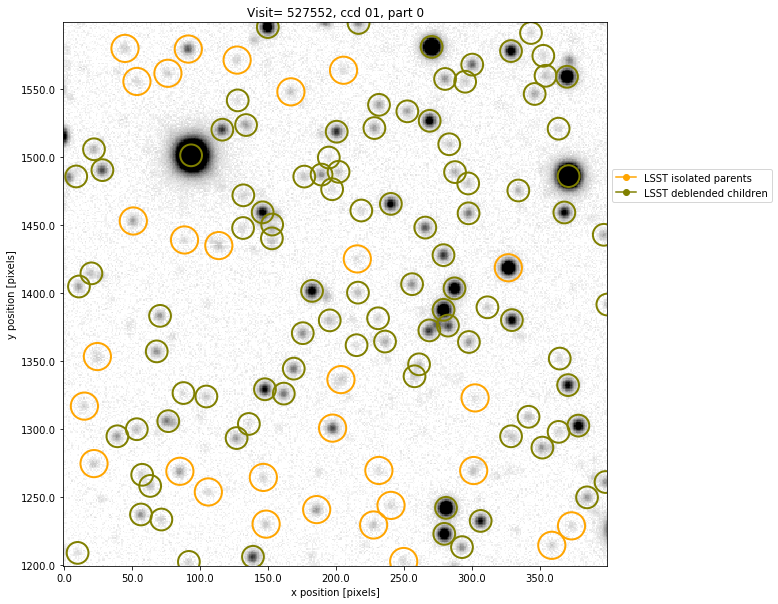
\includegraphics[width=1.0\columnwidth]{figs/visit_527552_ccd_1.png}
\caption{We illustrate the sources as reported by the LSST pipeline for a small region of CCD01 of visit 527552. A source may be reported as an isolated source (yellow),  or a successfully deblended child (green). In this analysis we only keep isolated parents or deblended children.}
\label{fig:lsst_sources}
\end{centering}
\end{figure} 




\section{Source detection and photometry}
\label{sec:metrics}

Starting with cleaned LSST and DECAPS source catalogs, we consider a set of metrics to compare the quality of LSST science pipelines to the  state-of-the-art DECAPS pipeline.  


We investigated bright, high S/N DECAPS sources that do not have an LSST match. We find that in most cases these sources in the LSST catalog have $S/N<5$ which led to their exclusion from the analysis (see Fig.~\ref{fig:lsst_decaps_sources}). We compare the count of  DECAPS to LSST sources in clean catalogs on Fig.~\ref{fig:lsst_count_comparison}. 

\begin{figure}
\begin{centering}
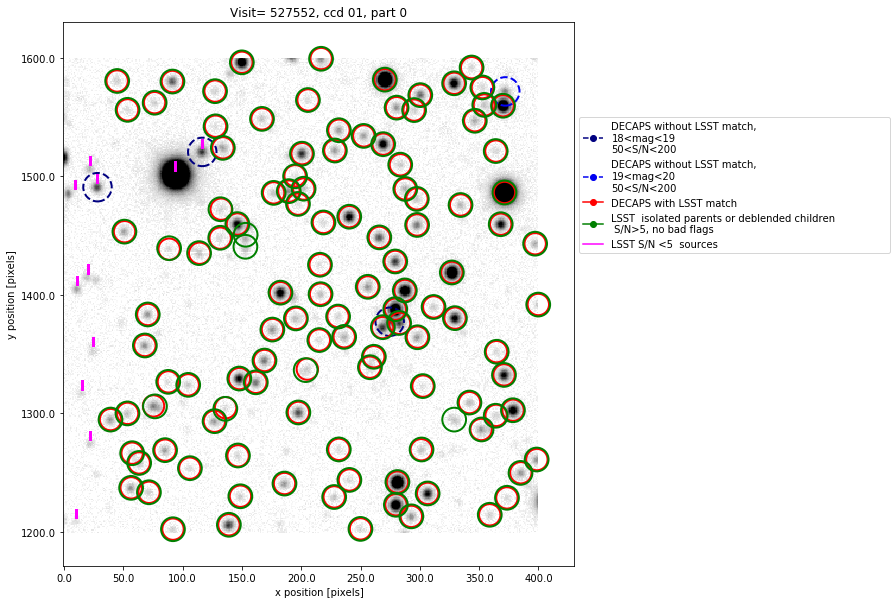
\includegraphics[width=1.1\columnwidth]{figs/visit_527552_ccd_1_lowSN.png}
\caption{The same region as on Fig.~\ref{fig:lsst_sources}. Green circles mark the position of retained LSST sources: isolated parents, or deblended children, with  S/N > 5, and no bad flags. Red circles mark the position of DECAPS detections with an LSST match. Vertical magenta dashes are above the LSST sources with S/N < 5.   Blue dashed circles mark location of DECAPS source without an LSST match. Note that eg. at (x,y) = 50,1490  an LSST source was detected, but since its  S/N < 5 it was not kept in the clean LSST catalog.   }
\label{fig:lsst_decaps_sources}
\end{centering}
\end{figure}



\begin{figure}
\begin{centering}
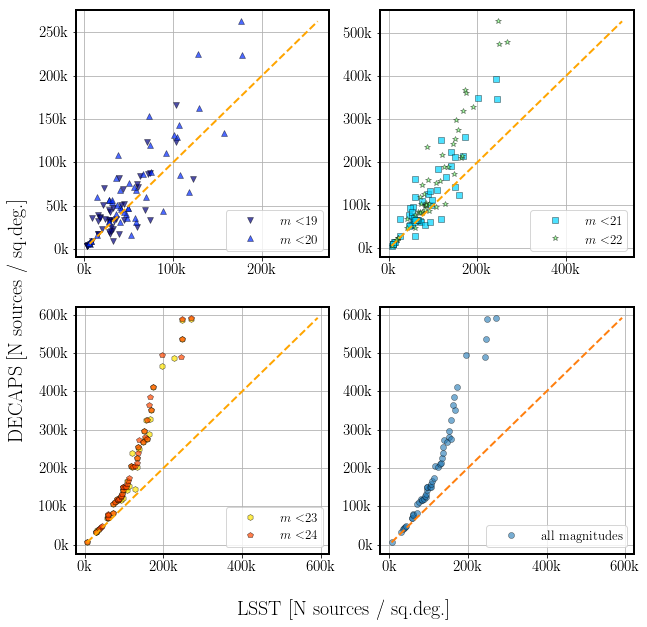
\includegraphics[width=0.9\columnwidth]{figs/decaps_lsst_source_count.png}
%\vskip -0.15in
\caption{A plot of source count comparing LSST to DECAPS source catalogs of the same fields (visits). 
On each panel we plot the number of counts up to a given magnitude, increasing the depth clockwise. 
The bottom right panel shows all sources without magnitude limits.}
\label{fig:lsst_count_comparison}
\end{centering}
\end{figure} 



% #############################################################
% ###################### completeness  ##########################
% #############################################################

\subsection{Completeness}

For each visit that corresponds to a given level of crowdedness, we consider the detection completeness of LSST to DECAPS. Assuming that DECAPS is the 'true' catalog of sources, we define completeness by the percentage of DECAPS sources (binned along DECAPS magnitude), that have an LSST match within 0.5 \arcsec. This is a very liberal requirement considering that for most visits >98\% of DECAPS sources have an LSST match within 0.3 \arcsec.  Second,  we require that the sources differ by not more than 0.5 magnitudes. As illustrated on Fig.~\ref{fig:dmag_scatter}, this only removes the outliers.  In fact, given that the majority of the sources (>99\%) that are matched within 0.5 \arcsec, do not differ by more than 0.5 magnitude, this constraint does not change the completeness by more than few \%.   Fig.~\ref{fig:completeness} shows how completeness , and catalog counts, depend on source density.


\begin{figure}
\begin{centering}
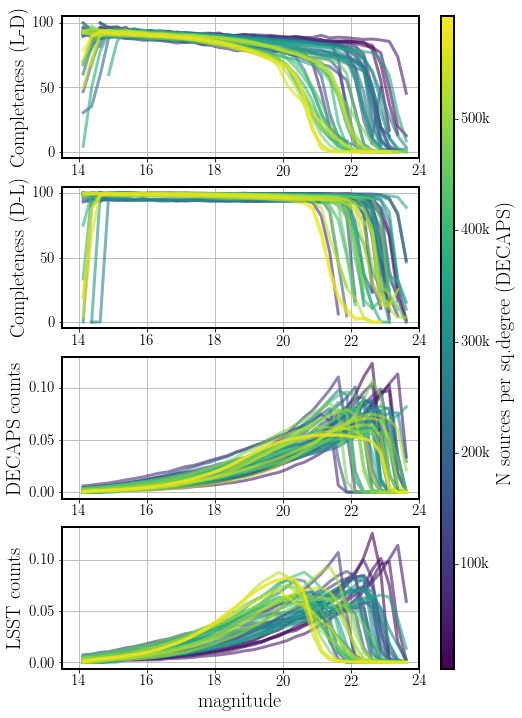
\includegraphics[width=0.75\columnwidth]{figs/completeness_4_panels_nomarker.png}
%\vskip -0.15in
\caption{Top two panels show source-to-source completeness.  The first panel is a measure of how complete is LSST catalog to DECAPS catalog (L-D),  i.e. the fraction of DECAPS sources per magnitude bin that have an LSST match.   The second panel shows an equivalent plot for the completeness of DECAPS to LSST (D-L), plotting the fraction of LSST sources that have a DECAPS match.  The bottom two panels show the normalized source counts  in the input catalogs. The LSST-DECAPS completeness falls off quicker than DECAPS-LSST, since DECAPS catalog has more sources at fainter magnitudes (see Fig.~\ref{fig:lsst_count_comparison}). Different colors correspond to different level of stellar crowdedness, expressed in terms of the number of sources per square degree in DECAPS clean catalogs.  We further characterize completeness by $\langle C_{18-20} \rangle$ - the mean completeness between 18-20 mag , and $m_{50}$ - the magnitude at which completeness falls to a 50\% level (see Fig.~\ref{fig:completeness_characterize}}
\label{fig:completeness}
\end{centering}
\end{figure} 


\begin{figure}
\begin{centering}
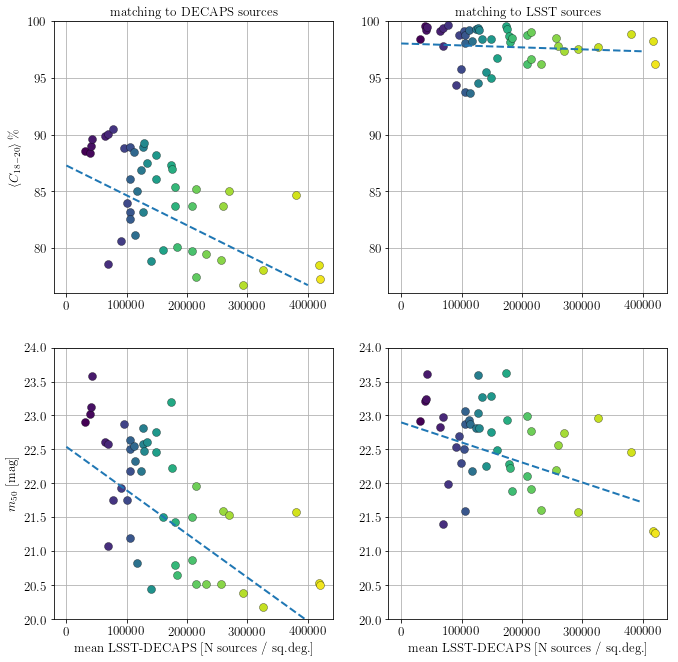
\includegraphics[width=0.96\columnwidth]{figs/decaps_lsst_c1820_m50.png}
%\vskip -0.15in
\caption{Magnitude at which completeness falls to 50\% (top two panels), and the mean completeness between 18 and 20 magnitudes (bottom two panels).  The panels on the left hand side correspond to the uppermost panel in Fig.~\ref{fig:completeness}, while the right hand side panels correspond to the second panel in Fig.~\ref{fig:completeness}. The color of all points corresponds to the stellar density, as in Fig.~\ref{fig:completeness}. In each panel we overplot the linear best-fit to indicate the expected overall trend of decreasing $\langle C_{18-20} \rangle$ and  $m_{50}$ with source density. }
\label{fig:completeness_characterize}
\end{centering}
\end{figure} 


\begin{figure}
\begin{centering}
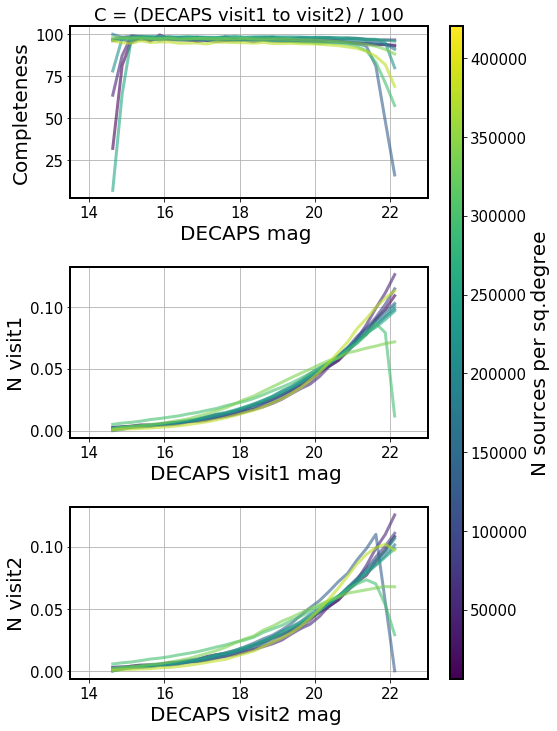
\includegraphics[width=0.75\columnwidth]{figs/completeness_3_decaps.png}
%\vskip -0.15in
\caption{The same quantities as on Fig.~\ref{fig:completeness}, but corresponding to two different visits at the same location, to test the repeatability of DECAPS detections. The two visits (visit1, visit2) were chosen in the same filter and at the same location, and as in tests for completeness, we match source-by-source and consider the number of sources per magnitude bin in visit1 that do have a matching source in visit2. }
\label{fig:completeness_decaps}
\end{centering}
\end{figure} 


% #############################################################
% ###################### PHOTOMETRY  ##########################
% #############################################################


\subsection{Photometry}
\label{sec:photometry}

We consider here photometric accuracy. Since both DECAPS and LSST processing pipelines start from the same instcal calibrated DECam images, they ought arrive at similar measurement of flux, and in turn, instrumental magnitudes.  

An offset and a spread in magnitude difference is due to details of each image processing pipeline.

We compare the photometric repeatability within each pipeline, as well as the existence of offset and spread between two different pipeines. We test pipeline repeatability by investigating two visits at the same locations,  taken in same filters, with equal exposure times.  Assuming that the majority of objects are non-variable in nature, we find the statistical epoch-to-epoch variance. 


\begin{figure}
\begin{centering}
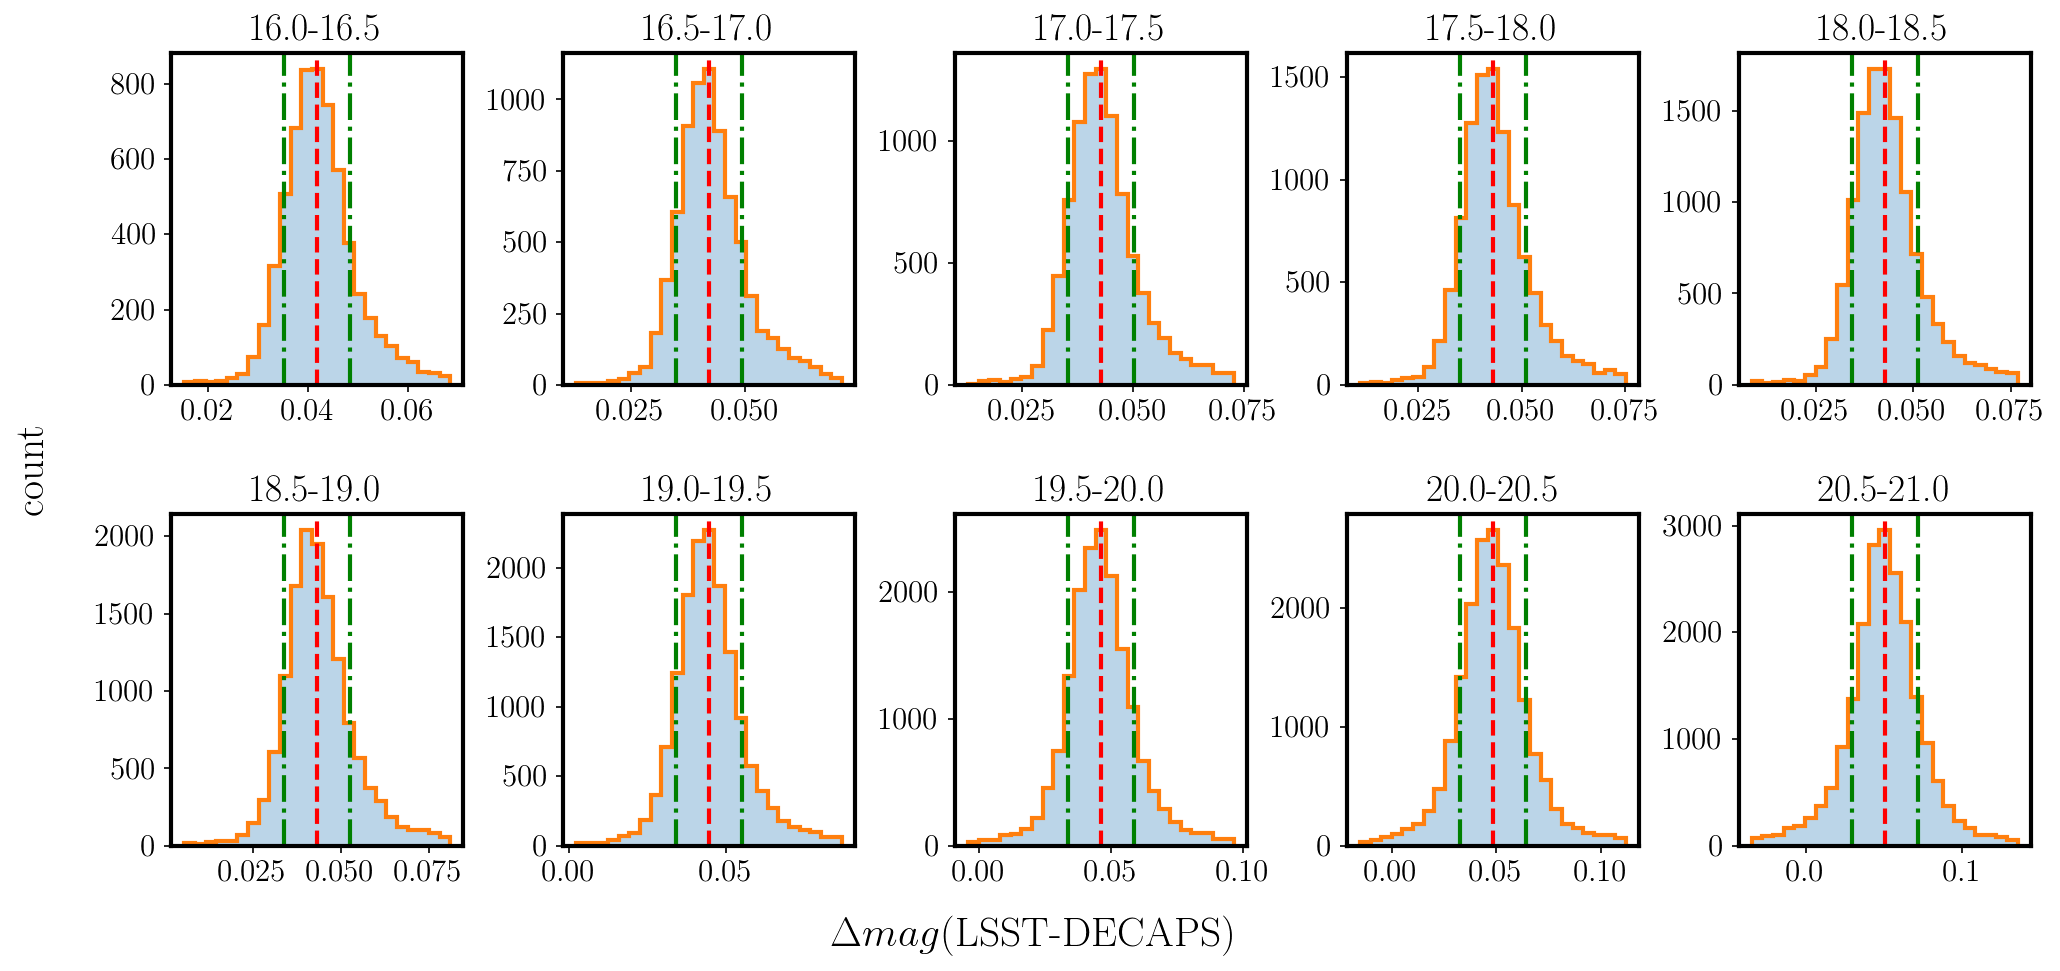
\includegraphics[width=1.1\columnwidth]{figs/rms_decaps_lsst_611970hist_panel.png}
%\vskip -0.15in
\caption{Cross-section of a difference in magnitudes between DECAPS and LSST for a visit 611970. Each panel contains the histogram of $\Delta mag$ per DECAPS magnitude bin. The vertical red line corresponds to the median value of $\Delta mag$ in that bin, and each histogram is limited between $\pm 4 \, \sigma_{G}$. THe vertical dot-dashed green lines mark the median $\pm \sigma_{G}$. }
\label{fig:dmag_hist}
\end{centering}
\end{figure} 


\begin{figure}
\begin{centering}
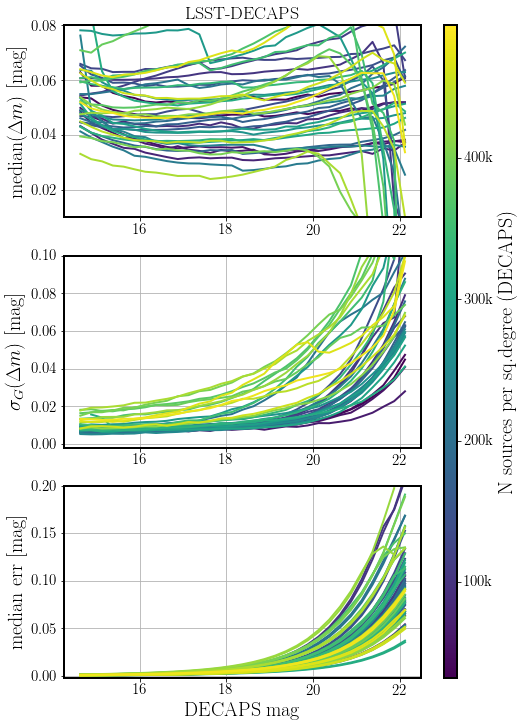
\includegraphics[width=0.7\columnwidth]{figs/decaps_lsst_rms_plot.png}
%\vskip -0.15in
\caption{The measurement of photometric offset between DECAPS and LSST pipelines. For each visit we cross-matched source catalogs corresponding to LSST and DECAPS processing; $\Delta m$ is the difference in magnitude reported between DECAPS and LSST for the same source. For each visit we bin sources according to their DECAPS magnitude. On three panels we plot the binned statistics : median($\Delta m$),  $\sigma_{G}(\Delta m)$, and median photometric uncertainty.}
\label{fig:lsst_decaps_dmag}
\end{centering}
\end{figure} 



Using the DECAPS image database for several visits we found a second visit at exactly the same location, filter and exposure time, but different epoch (see Table ~\ref{tab:epoch12_selection}).  This allowed to test the epoch-epoch photometric repeatability of DECAPS-LSST. We illustrate the  magnitude differences on Figs.~\ref{fig:decaps_decaps_dmag} and \ref{fig:lsst_lsst_dmag}, and the summary of the spread of photometric difference as a function of magnitude on Figs.~\ref{fig:epoch_lsst_multiplot} and ~\ref{fig:epoch_decaps_multiplot}. 




\begin{figure}
\begin{centering}
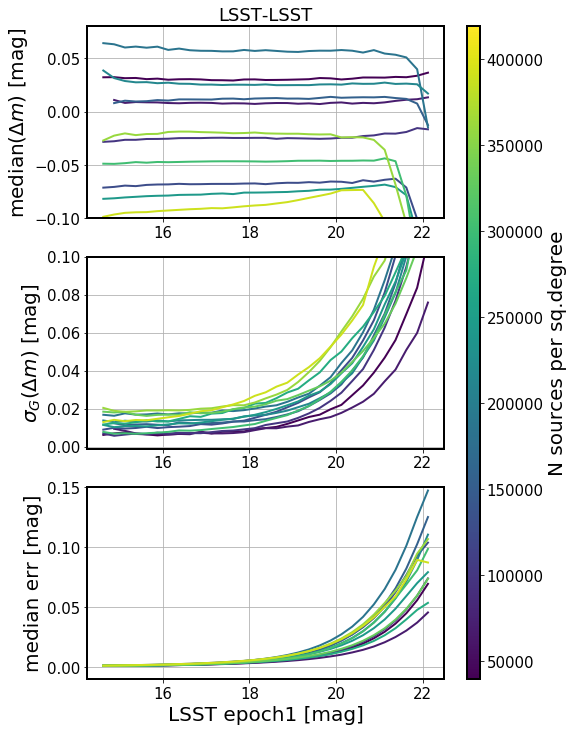
\includegraphics[width=0.8\columnwidth]{figs/lsst-lsst_rms_plot.png}
%\vskip -0.15in
\caption{The internal repeatability test of the LSST pipeline. We cross-match the source catalogs for each visit. These two brightness measurements for the same source are akin to a two-epoch light curve. Since inherently variable sources constitute a small fraction of all stellar objects, and the majority of stars are not variable, the difference in the measured magnitudes would correspond to the empirical measure of noise.  All sources cross-matched within 0.5\arcsec are binned according to their brightness. On the panels we plot, from top to bottom: median photometric offset, the robust interquartile-based measure of standard deviation $\sigma_{G}$, and the median reported measurement uncertainty.}
\label{fig:epoch_lsst_multiplot}
\end{centering}
\end{figure} 


\begin{figure}
\begin{centering}
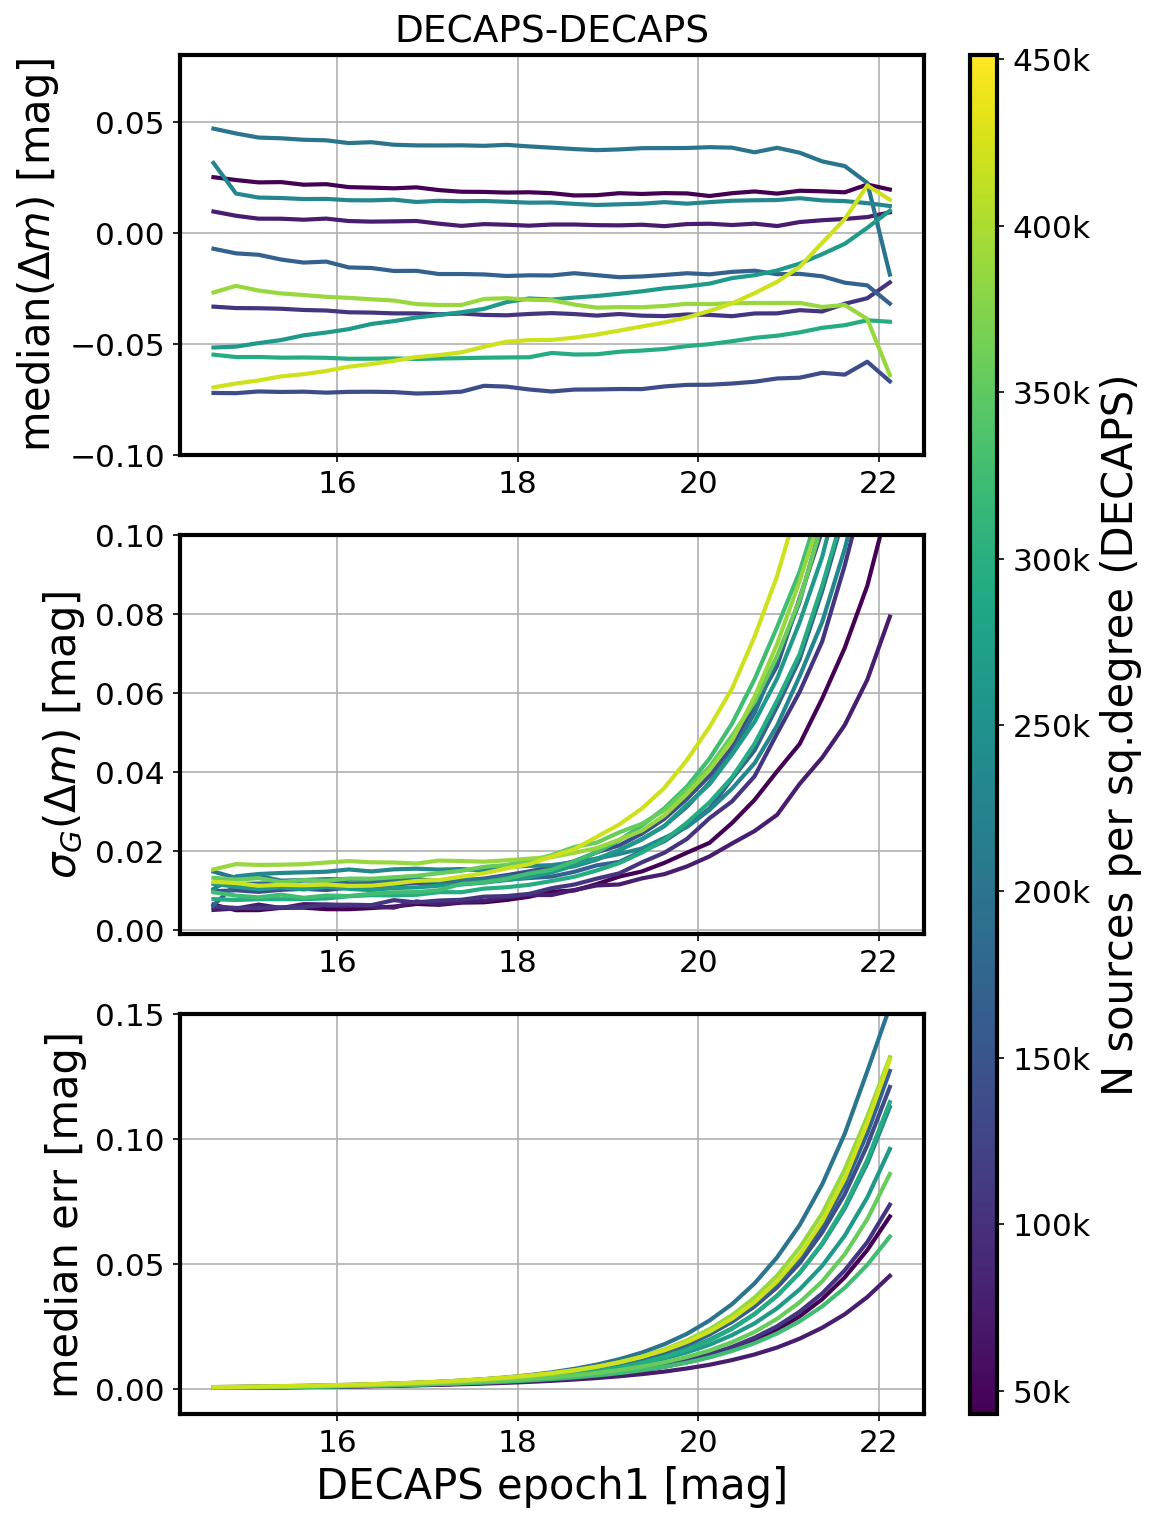
\includegraphics[width=0.8\columnwidth]{figs/decaps-decaps_rms_plot.png}
%\vskip -0.15in
\caption{The internal repeatability test of DECAPS pipeline - for description, see Fig.~\ref{fig:epoch_lsst_multiplot}.}
\label{fig:epoch_decaps_multiplot}
\end{centering}
\end{figure} 

We summarize the information about the photometric repeatability (epoch-to-epoch within a given pipeline), and offset (pipeline-to-pipeline of the same epoch), by combining information from  Figs.~\ref{fig:lsst_decaps_dmag},~\ref{fig:epoch_lsst_multiplot}, ~\ref{fig:epoch_decaps_multiplot}. 

On Fig.~\ref{fig:spread} and ~\ref{fig:spread_summary} we compare the spread of photometric scatter between the 
two pipelines and  the empirical measurement of noise from repeatability for a pair of visits at the same location. 

We consider visits  525846 and 530012, called epoch1 and epoch2. 

For each we first calculate the $\sigma_{G}(a,b)$  - the interquartile-based measure of spread of magnitude difference between measurements $a$ and $b$ of the same source. 

The spread of photometric scatter within the same pipeline, epoch-to-epoch: $\sigma_{G}(L1, L2)$, and $\sigma_{G}(D1,D2)$, correspond to the empirical measure of noise. 

$\sigma_{G}(L1, L2)$  is also plotted on the middle panel of Fig.~\ref{fig:epoch_lsst_multiplot}, while  $\sigma_{G}(D1,D2)$ is the same as that of Fig.~\ref{fig:epoch_decaps_multiplot}. 

The median error reported by either pipeline for either epoch is a measure of Poisson noise - the expected uncertainty in a repeated measurement. 

The scatter between the two pipelines calculated either for epoch1 or epoch2 :  $\sigma_{G}(D1,L1)$, or $\sigma_{G}(D2,L2)$). 


\begin{figure}
\begin{centering}
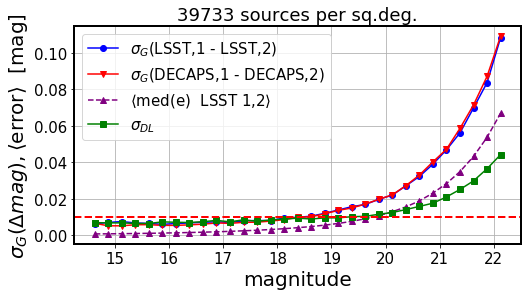
\includegraphics[width=0.8\columnwidth]{figs/photometric_spread_2_525846-530012.png}
%\vskip -0.15in
\caption{Analysis of  photometric spread. The solid blue and red lines of $\sigma_{G}$  represent the spread in photometry within each pipeline. The dashed purple line in the middle is the average reported error between the two epochs: a measure of Poisson noise. Finally, the bottom solid green line with square markers is the spread in photometry between the two pipelines.  Since LSST and DECAPS errors are almost identical, we choose to represent the minimum statistical offset by the mean LSST error between the two visits , added in quadrature . If $e_{1L}$ and $e_{2L}$ are LSST-reported error measurements for a given source for the two epochs,  the quadrature-mean is  $e_{12} = \sqrt{e_{1L}^{2} + e_{2L}^{2}} / \sqrt{2}$, and the purple dashed line is the median of $e_{12}$ per magnitude bin. We also add in quadrature the spread between the two pipelines: $\sigma_{DL,1}$ for epoch1, and $\sigma_{DL,2}$ for epoch2 : $\sigma_{DL} = \sqrt{\sigma_{DL,1}^{2} + \sigma_{DL,2}^{2}} / \sqrt{2}$.  Note that since the top blue (or red) lines $\sigma_{G}(LSST,1 - LSST,2)$, $\sigma_{G}(DECAPS,1 - DECAPS,2)$   ($\sigma_{DD}$, $\sigma_{LL}$ for short) consists of noise $\sigma_{E} $ and the systematic offset $\sigma_{S}$ : $\sigma_{LL}^{2} = \sigma_{S}^{2} + \sigma_{E}^{2}$. Thus we calculate the systematic offset for LSST as  $\sigma_{S} = \sqrt{\sigma_{LL}^2  - \sigma_{E}^{2}}$, which is the difference between  blue solid and purple dashed lines. 
}
\label{fig:spread}
\end{centering}
\end{figure} 



\begin{figure}
\begin{centering}
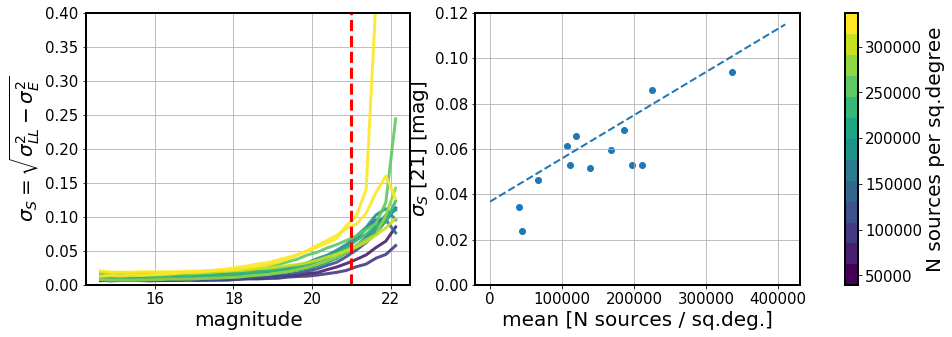
\includegraphics[width=0.95\columnwidth]{figs/photometric_offset_combined.png}
%\vskip -0.15in
\caption{The left panel shows the measure of systematic offset between mean photometric error, and the photometric repeatability for the LSST pipeline as a function of magnitude (see Figs.~\ref{fig:spread_1},~\ref{fig:spread_2}. The vertical line marks the level of 21 mag, at which we measure $\sigma_{S}$ :$\sigma_{S}[21]$. The right panel shows $\sigma_{S}[21]$  as a function of DECAPS stellar density.}
\label{fig:spread_summary}
\end{centering}
\end{figure} 

% #############################################################
% ###################### ASTROMETRY  ##########################
% #############################################################

\section{Astrometry}
\label{sec:astrometry}
Astrometry pertains to the measurement of the position of sources in the absolute World Coordinate System (WCS). Accurate and precise astrometry enables catalog cross-matching, and over long-term - measurement of proper motion of stellar sources. 

We consider two properties of successful astrometry. First, the internal consistency of a pipeline by measuring the repeatability of astrometric measurement between different epochs.  Second - accuracy, and any biases between the LSST-DECAPS pipelines. 

Part of the astrometric offset between the two pipelines is because  DECAPS employed 2MASS-GAIA data (Fig.12 in ~\cite{schlafly2017}), whereas LSST used GAIA data for astrometric calibration. 

To test the repeatability we use pairs of observations at the same location, as in Sec.~\ref{sec:photometry}. Fig.~\ref{fig:ra_dec_lsst_lsst} shows an example of the LSST-LSST comparison, with Fig.~\ref{fig:ra_dec_mag} showing the magnitude dependence. Fig.~\ref{fig:ra_dec_decaps_decaps} depicts the offset in $RA$, $DEC$, for DECAPS-DECAPS comparison. 


To test possible offset between LSST and DECAPS astrometric solutions, on Fig.~\ref{fig:ra_dec_lsst_decaps} we find the offset in measured $RA$, $DEC$ for sources cross-matched in catalogs from the two pipelines. 

\begin{figure}
\begin{centering}
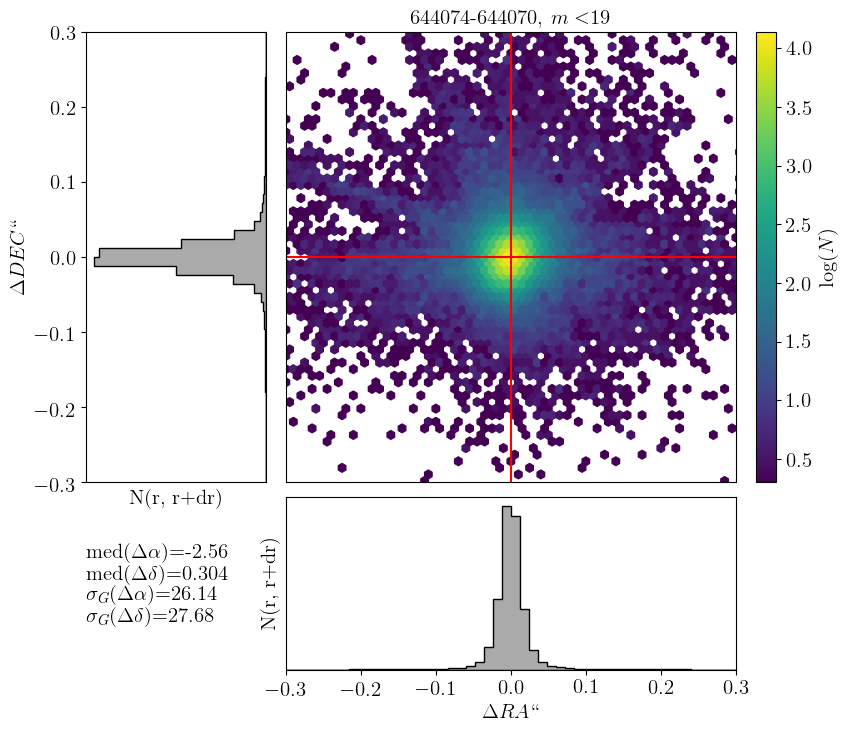
\includegraphics[width=0.8\columnwidth]{figs/lsst644074-644070_RA_DEC_offset_lims.png}
%\vskip -0.15in
\caption{The difference of LSST processing for  RA,DEC for visits 644074,644070: a pair of visits at the same location, separated by less than a day. The mean number of sources is 419000 sources per sq.deg., which corresponds to top 1\% of the sky.  We select sources brighter than 19 magnitude.  For all other pairs the  offsets are all centered on zero with similar spread - see Table~\ref{tab:radec_lsst_lsst}}
\label{fig:ra_dec_lsst_lsst}
\end{centering}
\end{figure} 


\begin{figure}
\begin{centering}
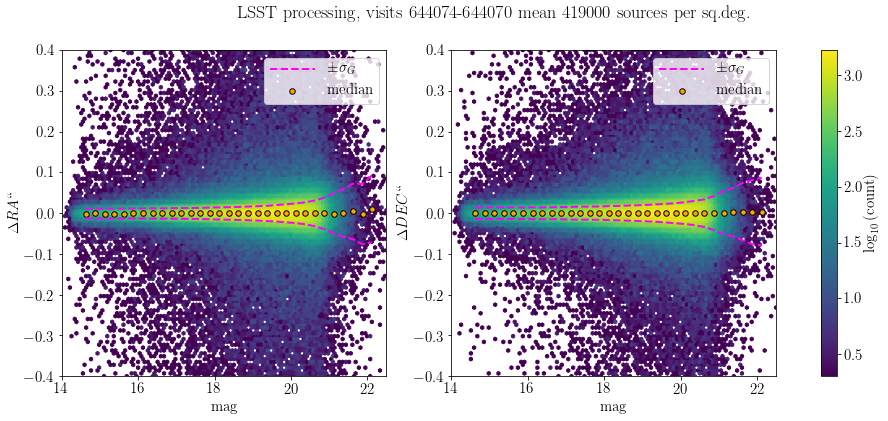
\includegraphics[width=1.0\columnwidth]{figs/644074-644070_dra_ddec_mag.png}
%\vskip -0.15in
\caption{The difference in RA,DEC for the same visits as on Fig.~\ref{fig:ra_dec_lsst_lsst}, shown as a function of magnitude.}
\label{fig:ra_dec_mag}
\end{centering}
\end{figure} 



\begin{figure}
\begin{centering}
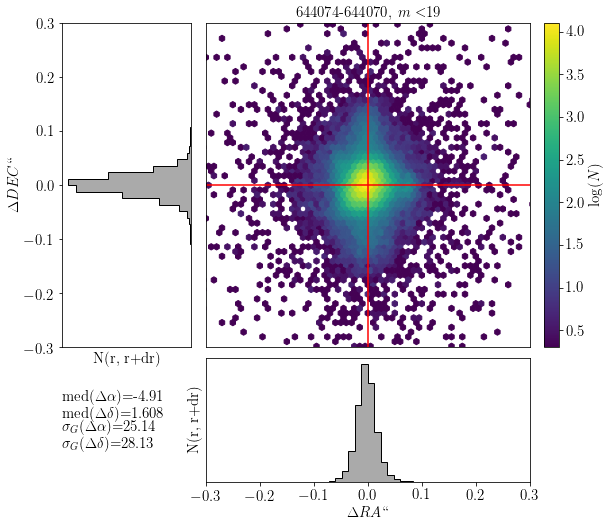
\includegraphics[width=0.8\columnwidth]{figs/decaps644074-644070_RA_DEC_offset_lims.png}
%\vskip -0.15in
\caption{The difference in RA,DEC for  the same visits as in Fig.~\ref{fig:ra_dec_lsst_lsst}, but comparing DECAPS single-epoch catalogs. The spread of  $\Delta \alpha$, $\Delta \delta$ is wider than for equivalent visit pairs processed by the LSST Science Pipelines - see Table~\ref{tab:radec_decaps_decaps}}
\label{fig:ra_dec_decaps_decaps}
\end{centering}
\end{figure} 




\begin{figure}
\begin{centering}
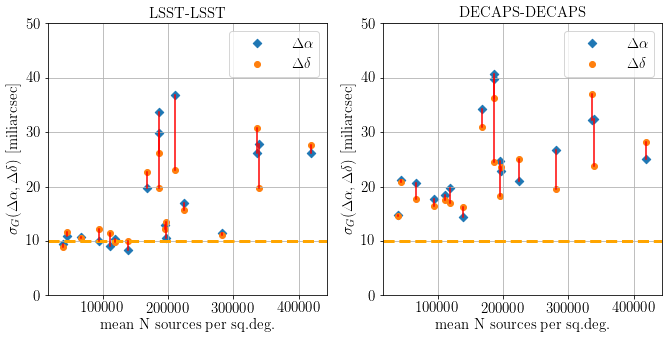
\includegraphics[width=0.8\columnwidth]{figs/Astrometry_LSST-LSST_DECAPS-DECAPS.png}
%\vskip -0.15in
\caption{Summary of LSST and DECAPS repeatability of astrometry, as in Tables ~\ref{tab:radec_lsst_lsst} and ~\ref{tab:radec_decaps_decaps}.}
\label{fig:lsst_decaps_side}
\end{centering}
\end{figure} 


\begin{figure}
\begin{centering}
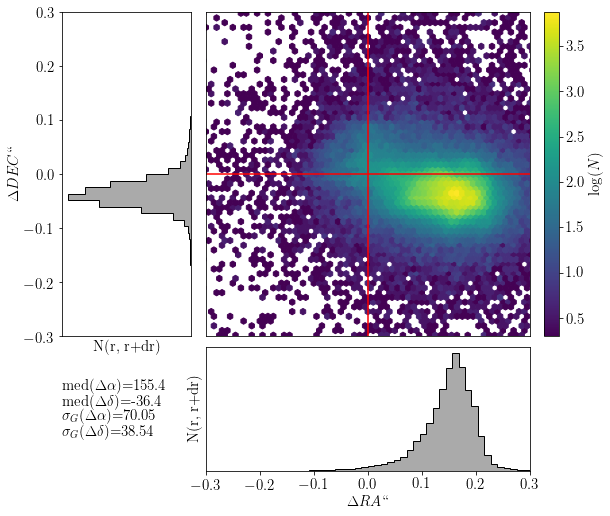
\includegraphics[width=0.8\columnwidth]{figs/22_525904_RA_DEC_offset.png}
%\vskip -0.15in
\caption{The difference in RA,DEC for visit 525904 , between LSST and DECAPS processing (402270 detected sources in  the clean LSST catalog ). We tested that for other vists and in all cases the offset position and magnitude remains the same - see Table~\ref{tab:radec_lsst_decaps}}
\label{fig:ra_dec_lsst_decaps}
\end{centering}
\end{figure} 



\section{Conclusions}
\label{sec:conclusions}

% ### need to add things here ... 

\subsection{LSST Processing of StarFast Simulated Sky}
An independent way to further test the performance of the LSST Science Pipelines is to use the simulated sky images, where the true position and  brightness of each source is known. This would put the measure of source detection completeness, photometric and astrometric precision on an absolute scale. We already tested a StarFast image simulator\footnote{\url{https://dmtn-012.lsst.io}}, and confirmed that it can successfully simulate a region of the sky seeded with known stellar population.  


\subsection{Other LSST-DECAPS tests: w-color }
An independent test of the quality of photometry would be to consider the width of the stellar locus ('w-color') on the g-r vs r-i color-color plot.  This could be used to test internal consistency of LSST and DECAPS photometry. 



%%%%%%%%%%%%%%%%%%%%%%%%%%%%%%%%%%%%%%%%%%%%%%%%%%
%%%%%%%%%%%%%%%%%%%% REFERENCES %%%%%%%%%%%%%%%%%%
%%%%%%%%%%%%%%%%%%%%%%%%%%%%%%%%%%%%%%%%%%%%%%%%%%

\bibliographystyle{apj}
\bibliography{references}
\end{document}